En esta sección de la investigación, se exponen antecedentes relacionados con la identificación y el prediagnóstico de nódulos en diferentes órganos mediante diversas metodologías. Estos antecedentes servirán para comprender el enfoque y establecer fundamentos sólidos para el adecuado desarrollo del presente proyecto.

\cite{Zhao2024} desarrollaron un modelo de clasificación avanzado denominado Swin-ResNet, orientado a la identificación de marcas dentales en la lengua, con el propósito de mejorar la precisión y objetividad en el diagnóstico de deficiencias del bazo en la medicina tradicional china. Este modelo combina las capacidades de la red neuronal convolucional ResNet-50 con el transformador Swin, un tipo de arquitectura que permite una extracción de características más eficiente y precisa. La integración de estos dos enfoques tiene como objetivo optimizar la detección de marcas dentales que son difíciles de percibir a simple vista, lo cual es crucial para un diagnóstico más certero en los pacientes.

El modelo fue entrenado utilizando un conjunto de 1.500 imágenes clínicas de la lengua, obtenidas del Hospital ShuGuang, afiliado a la Universidad de Medicina Tradicional China de Shanghai. Estas imágenes fueron procesadas utilizando una arquitectura de convoluciones de tamaño 7×7, combinada con módulos Swin-T, los cuales son fundamentales para la extracción de características de alto nivel. La evaluación del rendimiento del modelo reveló una notable precisión promedio de 0.9959 en la clasificación de las imágenes de la lengua, dividiéndolas en tres categorías: marcas leves, sin marcas y marcas severas. Estos resultados posicionaron al modelo Swin-ResNet por encima de otros enfoques populares como EfficientNet-v2 y RegNet, que mostraron precisiones inferiores de 0.8038 y 0.8796, respectivamente. Además, aunque Swin Transformer tiene más parámetros, el modelo Swin-ResNet demostró ser más eficiente y rápido en esta tarea, destacándose por su capacidad para realizar diagnósticos automatizados con un alto grado de precisión.

Estos resultados subrayan la eficacia del modelo Swin-ResNet en el ámbito de la medicina tradicional china, específicamente en el diagnóstico de marcas dentales en la lengua, brindando una herramienta confiable y precisa para mejorar la atención médica en este campo.

La metodologia a emplearse para este trabajo fue la siguiente y se puede observar en la Figura \ref{2:fig123}.

\begin{figure}[H]
	\begin{center}
		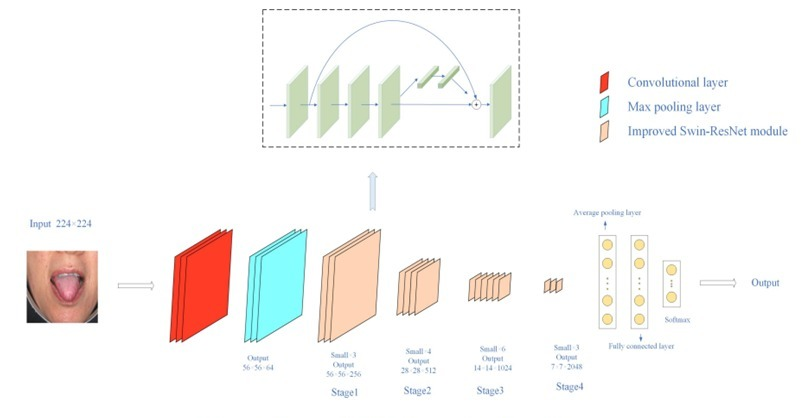
\includegraphics[width=0.80\textwidth]{2/figures/1.jpeg}
		\caption[Metodologia ResNet-50 and Swin Transformer]{Metodologia ResNet-50 and Swin Transformer. \\
		Fuente: \cite{Zhao2024}. \textit{Swin-ResNet: Research and Implementation of a Tooth-Marked
		Tongue Classification Method Combining ResNet-50 and Swin Transformer.}.}
		\label{2:fig123}
	\end{center}
\end{figure}

\cite{Tang2020} desarrollaron un enfoque innovador basado en aprendizaje profundo para la detección automática de lenguas con marcas de dientes, un elemento crucial en el diagnóstico dentro de la medicina tradicional china. El reto principal en este campo radica en la variabilidad de las características visibles de la lengua, particularmente en las marcas dejadas por los dientes en los bordes de la lengua, lo que requiere una metodología de clasificación altamente detallada y precisa. Para abordar este desafío, el equipo implementó una red neuronal convolucional en cascada, compuesta por tres etapas: coarse-Net, fine-Net y refine-Net, que trabajan conjuntamente para detectar y localizar la región de la lengua y los puntos de referencia clave asociados a las marcas dentales. Posteriormente, se emplearon redes ResNet-50 y VGG-16 para llevar a cabo una clasificación precisa de las imágenes de la lengua.

El conjunto de datos utilizado para entrenar y validar este modelo incluyó un total de 1,858 imágenes de lenguas, obtenidas del Hospital Afiliado de la Universidad de Medicina Tradicional China de Chengdu. La implementación de este sistema de aprendizaje profundo mostró una mejora significativa en las métricas de evaluación, superando los enfoques tradicionales que no emplean aprendizaje profundo en cuanto a precisión y consistencia con la percepción humana. El F1-score, que es una medida clave en la evaluación de modelos de clasificación, alcanzó un valor de 0.924 al utilizar ResNet-50, y mejoró aún más a 0.948 cuando se utilizó VGG-16. Estos resultados demostraron que la inclusión de la localización de la región de la lengua y los puntos de referencia de la lengua mejoró significativamente la precisión del modelo.

Este trabajo no solo resalta el potencial del aprendizaje profundo en el ámbito de la medicina tradicional china, sino que también establece un nuevo estándar en la clasificación de lenguas con marcas dentales, destacándose por su capacidad para realizar diagnósticos más rápidos y precisos que los métodos convencionales. La propuesta de \cite{Tang2020} representa un avance pionero en la integración de tecnologías avanzadas de reconocimiento visual para la mejora de diagnósticos médicos en este campo.

La metodología que se empleó para este trabajo fue la siguiente y se puede observar en la Figura \ref{2:fig124}.

\begin{figure}[H]
	\begin{center}
		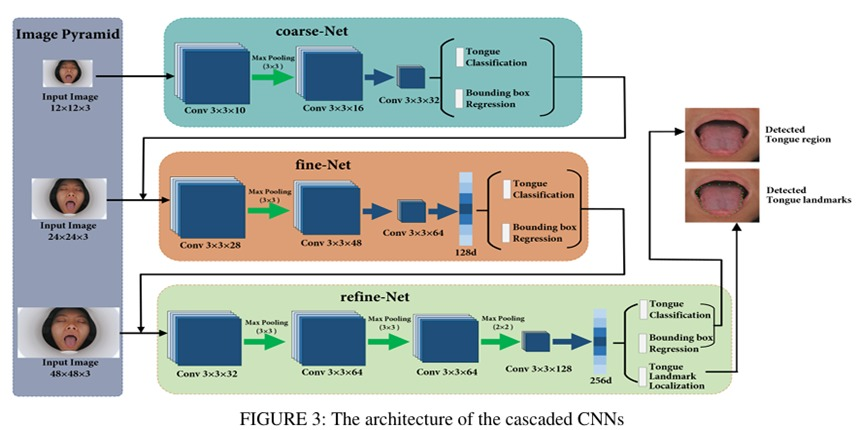
\includegraphics[width=0.80\textwidth]{2/figures/2.jpeg}
		\caption[Metodología ResNet-50 y VGG-16]{Metodología ResNet-50 y VGG-16. \\
		Fuente: \cite{Tang2020}. \textit{An Automatic Recognition of Tooth-Marked Tongue Based on Tongue Region Detection and Tongue Landmark Detection via Deep Learning.}.}
		\label{2:fig124}
	\end{center}
\end{figure}

La investigación llevada a cabo por \cite{Jiatuo2024} aborda el uso de algoritmos de aprendizaje profundo en el análisis y diagnóstico de imágenes de la lengua, un campo crucial en la medicina tradicional china (TCM). Este estudio se centra en el empleo del dataset público BioHit, que contiene 300 imágenes clínicas de lenguas, como base para la experimentación. A través del uso de redes neuronales convolucionales (CNNs) y técnicas de aprendizaje clásico, los autores lograron establecer un marco analítico que combina segmentación, detección de lesiones y clasificación automática de características presentes en las imágenes de lengua.  

En cuanto a la metodología, los investigadores implementaron una red neuronal profunda basada en CNN para extraer características específicas de las imágenes, enfocándose en patrones distintivos como marcas dentales, irregularidades en la textura y variaciones en el revestimiento de la lengua. Este enfoque permitió no solo identificar lesiones con precisión, sino también segmentar regiones clave de interés dentro de las imágenes. Paralelamente, se exploraron modelos clásicos para contrastar los resultados obtenidos con las técnicas más avanzadas.

El estudio reportó resultados significativos al comparar los enfoques clásicos con los de aprendizaje profundo. Mientras que los métodos convencionales alcanzaron una precisión aproximada del 80\% en la detección de lenguas marcadas por dientes, los modelos de aprendizaje profundo lograron precisiones mucho más altas, variando entre el 88\% y el 98.94\%. Entre los modelos más destacados se encuentran ResNet34, con una precisión máxima de 91.47\%, y una red neuronal convolucional multitarea, que alcanzó una precisión sobresaliente del 98.94\%. Este trabajo resalta cómo las técnicas basadas en inteligencia artificial no solo superan a los métodos tradicionales, sino que también aportan un nivel de estandarización y precisión nunca antes visto en el diagnóstico visual en TCM, abriendo nuevas posibilidades para el uso clínico de estas tecnologías.

La metodología seguida en este trabajo puede observarse en la Figura \ref{2:fig125}, la cual resume el proceso desde la segmentación inicial hasta la clasificación final basada en redes neuronales profundas.

\begin{figure}[H]
	\begin{center}
		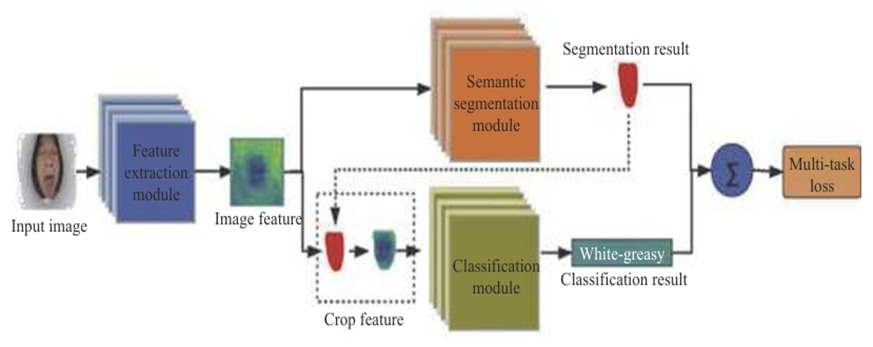
\includegraphics[width=0.80\textwidth]{2/figures/3.jpeg}
		\caption[Metodología de análisis de imágenes de lengua con CNNs]{Metodología de análisis de imágenes de lengua con CNNs. \\
		Fuente: \cite{Jiatuo2024}. \textit{Research status and prospect of tongue image diagnosis analysis based on machine learning.}.}
		\label{2:fig125}
	\end{center}
\end{figure}

En el trabajo de \cite{Liu2023}, se presenta un análisis exhaustivo sobre el uso de la inteligencia artificial en el diagnóstico médico mediante imágenes de lengua, un área relevante en la medicina tradicional china (TCM). A través de una revisión de los estudios más recientes publicados en bases de datos científicas como Web of Science y IEEE en los últimos cinco años, los autores destacan la evolución y los resultados prometedores obtenidos mediante la aplicación de algoritmos de aprendizaje profundo y técnicas híbridas. Este enfoque ha permitido avances significativos en la segmentación, detección y clasificación de imágenes de lengua, optimizando su uso en la diferenciación de síndromes y el diagnóstico de enfermedades.  

La metodología empleada se basa principalmente en el uso de redes neuronales convolucionales (CNNs) y modelos híbridos que integran inteligencia artificial con principios de TCM. Los modelos investigados incluyen técnicas avanzadas como ResNet50 y XGBT optimizado, los cuales se utilizaron para tareas específicas como la calibración y segmentación precisa de regiones de interés en las imágenes de lengua. Además, se destaca la implementación de modelos multitarea, como U-Net, que mejoraron significativamente la capacidad de detección y clasificación de lesiones, incrementando la eficiencia del diagnóstico.  

En términos de resultados, los modelos de aprendizaje profundo lograron precisiones que oscilan entre el 85\% y el 98\% en segmentación y clasificación de enfermedades a partir de imágenes de lengua. Por ejemplo, ResNet50 mostró una precisión de hasta el 92\% en la identificación de condiciones como prediabetes y diabetes. Por otro lado, los modelos híbridos, como un XGBT optimizado, alcanzaron un rendimiento máximo de 98\%, superando a métodos tradicionales en múltiples aspectos. Estas cifras resaltan la capacidad de la inteligencia artificial para transformar el diagnóstico médico al ofrecer mayor precisión y consistencia en los análisis visuales.

Pese a estos avances, los autores también subrayan desafíos importantes que persisten en esta área. Entre ellos se encuentran la necesidad de construir conjuntos de datos más completos y diversos, así como garantizar la fiabilidad en la evaluación de resultados. Además, se menciona que las futuras investigaciones deberían enfocarse en métodos de auto-supervisión y la fusión multimodal de datos, que permitirían una integración más robusta y precisa de la inteligencia artificial en los procesos de diagnóstico médico. Este trabajo establece una base sólida para el desarrollo continuo de tecnologías de diagnóstico inteligente basadas en imágenes de lengua, alineando la medicina tradicional con herramientas modernas de análisis.  

La metodología analizada en este estudio se ilustra en la Figura \ref{2:fig126}, la cual detalla el flujo de trabajo desde la segmentación inicial hasta la clasificación utilizando redes neuronales y modelos híbridos.

\begin{figure}[H]
	\begin{center}
		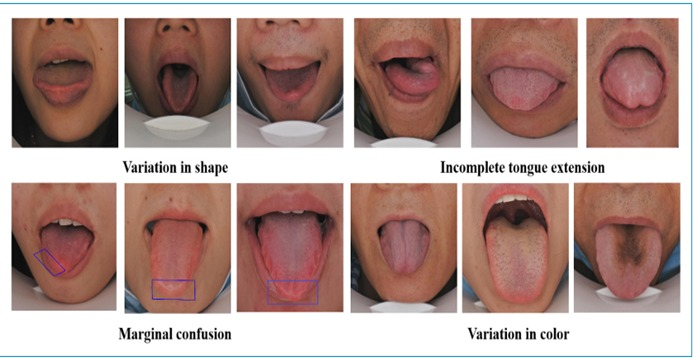
\includegraphics[width=0.80\textwidth]{2/figures/4.jpeg}
		\caption[Enfoque metodológico en el análisis de imágenes de lengua]{Enfoque metodológico en el análisis de imágenes de lengua utilizando modelos híbridos. \\
		Fuente: \cite{Liu2023}. \textit{A survey of artificial intelligence in tongue image for disease diagnosis and syndrome differentiation.}.}
		\label{2:fig126}
	\end{center}
\end{figure}

El estudio realizado por \cite{Jiang2022} examina la aplicación de algoritmos de aprendizaje profundo para el análisis de imágenes de lengua, integrando conocimientos de la medicina tradicional china (TCM). Con un conjunto de datos compuesto por 8,676 imágenes, estas fueron clasificadas en siete categorías distintas: lengua fisurada, marcada por dientes, estasis, con manchas, recubrimiento graso, pelada y podrida. Estas imágenes fueron recopiladas y anotadas por expertos en TCM, lo que garantiza la precisión y relevancia de los datos utilizados.  

La metodología principal implementada en este estudio se basa en el modelo Faster R-CNN, combinado con ResNet101 como extractor de características. Este enfoque permitió la detección y clasificación multietiqueta de las imágenes de lengua con un alto nivel de detalle. Para entrenar el modelo, las imágenes se dividieron en conjuntos de entrenamiento, validación y prueba, y se ejecutaron en un entorno optimizado con GPUs para acelerar los procesos de cálculo. Esta configuración permitió identificar patrones específicos en las imágenes, vinculándolos con características fisiológicas relevantes.  

En cuanto a los resultados, el modelo logró un desempeño destacado, alcanzando una precisión promedio del 90.67\%, una precisión puntual del 99.28\%, un recall del 91.25\% y un F1-score del 95.00\%. Estos indicadores destacan la capacidad del modelo para identificar con precisión características complejas y relevantes en las imágenes de lengua. Además, en una aplicación diagnóstica más amplia, el modelo identificó características específicas en una población de análisis, como lenguas fisuradas (41.49\%), marcadas por dientes (37.16%) y con recubrimiento graso (29.66\%).  

Más allá de la clasificación precisa, el estudio reveló asociaciones significativas entre las características de la lengua y ciertas condiciones metabólicas, como hipertensión, sobrepeso y enfermedades relacionadas con el hígado graso no alcohólico (NAFLD). Estas correlaciones sugieren que las características visibles de la lengua pueden ser indicadores valiosos para diagnósticos tempranos en diversas enfermedades. Asimismo, se identificaron variaciones en la prevalencia de estas características según el género y la edad de los individuos, lo que subraya la importancia de personalizar los análisis diagnósticos.  

\begin{figure}[H]
	\begin{center}
		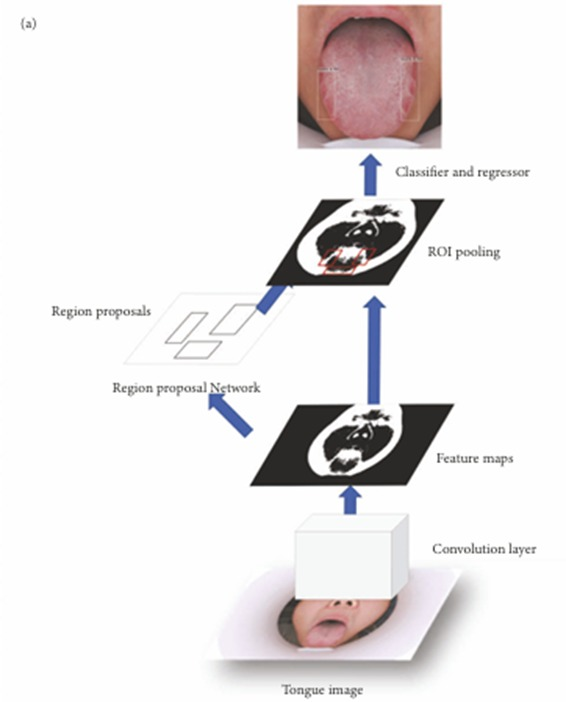
\includegraphics[width=0.7\textwidth]{2/figures/5.jpeg}
		\caption[Metodología con Faster R-CNN y ResNet101]{Metodología con Faster R-CNN y ResNet101 para el análisis de imágenes de lengua. \\
		Fuente: \cite{Jiang2022}. \textit{Deep learning analysis of tongue images in traditional Chinese medicine diagnosis.}.}
		\label{2:fig127}
	\end{center}
\end{figure}

El estudio presentado por \cite{Feasibility2020} analiza la viabilidad de Google’s Teachable Machine (versión 2.0) como herramienta de aprendizaje automático para el diagnóstico de lenguas marcadas por dientes, una característica comúnmente asociada con diversas afecciones de salud bucal. Utilizando un conjunto de datos de 1,250 imágenes obtenidas de Kaggle, el estudio incluye 704 imágenes de lenguas con marcas de dientes y 546 sin marcas, recopiladas y etiquetadas para garantizar su adecuación en aplicaciones diagnósticas.

La metodología se centró en optimizar el rendimiento del modelo ajustando hiperparámetros clave como el número de épocas, el tamaño del lote y la tasa de aprendizaje. El conjunto de datos se dividió en un 90\% para entrenamiento y un 10\% para pruebas, asegurando un adecuado equilibrio entre generalización y precisión. Google’s Teachable Machine, diseñada para simplificar la implementación de modelos de aprendizaje automático, fue utilizada como herramienta base, demostrando que su interfaz accesible puede integrarse en flujos de trabajo clínicos para diagnóstico.

Los resultados obtenidos muestran que el modelo logró una precisión del 92.1\% en la identificación de lenguas marcadas por dientes, mientras que para lenguas sin marcas alcanzó un 72.6\%. La sensibilidad del modelo fue de 0.92, destacando su capacidad para detectar correctamente casos positivos, aunque la especificidad fue baja (0.28), indicando limitaciones en la identificación de casos negativos. Este rendimiento supera al de estudios previos basados en redes neuronales convolucionales más complejas, lo que subraya la efectividad de herramientas accesibles como Teachable Machine en contextos clínicos.

Estos hallazgos no solo resaltan la capacidad de esta herramienta para realizar diagnósticos con una precisión competitiva, sino que también abren la puerta a nuevas aplicaciones en entornos con recursos limitados, donde el acceso a infraestructura avanzada de aprendizaje profundo es restringido. Además, el enfoque simplificado de Google’s Teachable Machine facilita la adopción de tecnologías de inteligencia artificial en la práctica médica, permitiendo a los profesionales implementar soluciones rápidas y eficientes para el diagnóstico de condiciones clínicas.

\begin{figure}[H]
	\begin{center}
		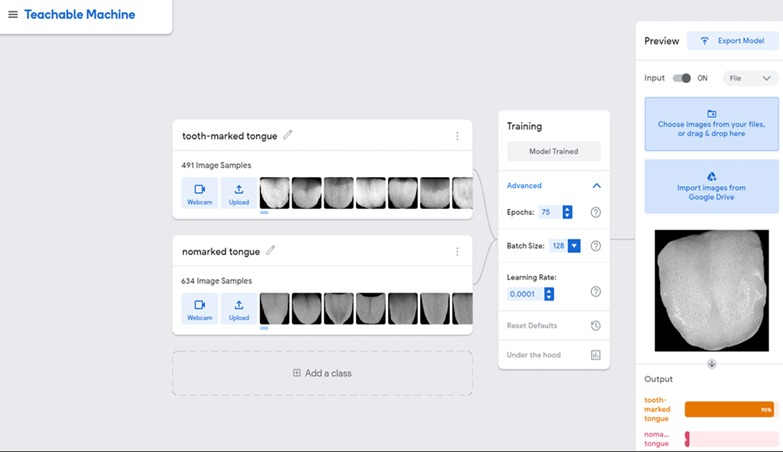
\includegraphics[width=0.80\textwidth]{2/figures/6.jpeg}
		\caption[Flujo de trabajo en Google’s Teachable Machine]{Flujo de trabajo para diagnóstico de lengua marcada por dientes utilizando Google’s Teachable Machine. \\
		Fuente: \cite{Feasibility2020}. \textit{Feasibility Study of Google's Teachable Machine in Diagnosis of Tooth-Marked Tongue.}.}
		\label{2:fig128}
	\end{center}
\end{figure}

El estudio de \cite{Kong2020} presenta una metodología avanzada para la detección y análisis de lenguas marcadas por dientes, un rasgo distintivo en el diagnóstico de la medicina tradicional china (TCM), que puede estar asociado con disfunciones en órganos internos como el hígado y el bazo. Este trabajo se basa en un conjunto de datos compuesto por 1,500 imágenes clínicas de alta calidad provenientes del Hospital Shu Guang en Shanghái. Dentro de este conjunto, se seleccionaron específicamente 400 imágenes de lenguas normales y 756 con marcas de dientes, las cuales fueron etiquetadas manualmente para garantizar la precisión en la segmentación y localización de las marcas.

La metodología empleada combina el poder del modelo Mask Scoring R-CNN con técnicas de aprendizaje por transferencia, utilizando ResNet-101 como red base. Este enfoque permitió una segmentación precisa y una localización detallada de las marcas dentales presentes en las imágenes. Antes del entrenamiento del modelo, las imágenes fueron sometidas a un proceso de preprocesamiento intensivo, incluyendo la normalización del color, recorte y etiquetado manual de las áreas de interés para generar máscaras altamente detalladas. Estos pasos fueron fundamentales para optimizar la detección de marcas dentales, especialmente en casos con grados de severidad diversos.

Los resultados del estudio fueron sobresalientes. El modelo alcanzó un F1-score de 0.95, lo que refleja un equilibrio casi perfecto entre precisión y recall. Además, la precisión específica del modelo fue del 99\%, mientras que el recall alcanzó un valor notable de 91.4\%. Estos indicadores demuestran no solo la alta precisión del modelo, sino también su capacidad para generalizar en diferentes escenarios clínicos. Esto es particularmente relevante dado que las lenguas marcadas por dientes pueden variar significativamente en términos de su apariencia y severidad.

Una de las contribuciones más destacadas de esta investigación es su aplicabilidad en el ámbito de la telemedicina. Al integrar herramientas avanzadas de aprendizaje profundo como Mask Scoring R-CNN, se abre la posibilidad de realizar diagnósticos detallados a distancia, reduciendo la dependencia de evaluaciones presenciales y facilitando el acceso a servicios médicos especializados. Esto es especialmente relevante en áreas donde la medicina tradicional china es una práctica común, pero los recursos médicos pueden ser limitados.

\begin{figure}[H]
	\begin{center}
		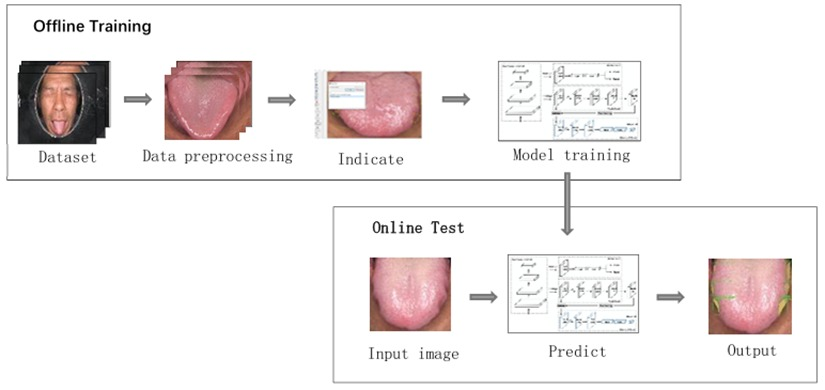
\includegraphics[width=0.80\textwidth]{2/figures/7.jpeg}
		\caption[Detección de lengua marcada por dientes con Mask Scoring R-CNN]{Esquema de segmentación y localización de marcas dentales utilizando Mask Scoring R-CNN con ResNet-101. \\
		Fuente: \cite{Kong2020}. \textit{Tooth-marked tongue recognition based on Mask Scoring R-CNN.}}
		\label{2:fig129}
	\end{center}
\end{figure}

Este estudio subraya la relevancia de la inteligencia artificial en la modernización de los diagnósticos basados en imágenes, mostrando cómo modelos avanzados pueden superar las limitaciones tradicionales de precisión y consistencia en el análisis de características complejas como las marcas de dientes en la lengua.

El trabajo de \cite{Tiryaki2024} explora el uso de redes neuronales profundas (DCNN) en la identificación y clasificación de lesiones en la lengua, un campo emergente con importantes aplicaciones clínicas. Este estudio aborda específicamente cinco categorías: lengua normal y cuatro tipos de lesiones comunes, incluyendo lengua fisurada, lengua geográfica, lengua recubierta y glositis romboidal mediana. Para este análisis, se recopiló un conjunto de datos compuesto por 623 imágenes clínicas de lengua, etiquetadas de manera experta para garantizar la precisión en la categorización.

La metodología implementada incluyó el uso de varios modelos avanzados de DCNN, como VGG19, ResNet50, ResNet101 y GoogLeNet. Estos modelos se beneficiaron del aprendizaje por transferencia, una técnica que aprovecha redes preentrenadas para mejorar la eficiencia en problemas con datos limitados. Además, este estudio introdujo por primera vez en este contexto un enfoque innovador basado en la fusión por votación mayoritaria (FBMV, por sus siglas en inglés), diseñado para combinar las predicciones de múltiples modelos y mejorar la precisión global.

Los resultados obtenidos fueron notables tanto en la clasificación binaria como en la clasificación multiclase. En la tarea binaria (lengua normal vs. lengua con lesiones), el modelo ResNet101 logró una precisión inicial del 93.53\%. Este rendimiento fue mejorado significativamente mediante la aplicación del enfoque FBMV, alcanzando un 95.15\%. Para la clasificación multiclase, que abarcó las cinco categorías, VGG19 se destacó con una precisión del 83.93\%, la cual fue incrementada al 88.76\% tras incorporar FBMV. Estos resultados no solo demuestran la robustez de las redes neuronales profundas en la detección de características complejas de la lengua, sino también el valor añadido del enfoque de fusión para abordar problemas de clasificación con múltiples clases.

Además de los resultados cuantitativos, el estudio subraya el potencial de estas tecnologías en el ámbito clínico. La capacidad de las DCNN para identificar patrones sutiles y correlaciones en imágenes médicas abre nuevas posibilidades para diagnósticos automatizados y personalizados. Este avance es especialmente relevante en entornos con recursos limitados, donde las herramientas basadas en inteligencia artificial pueden complementar la experiencia de los profesionales de la salud, mejorando la eficiencia y reduciendo los tiempos de diagnóstico.

\begin{figure}[H]
	\begin{center}
		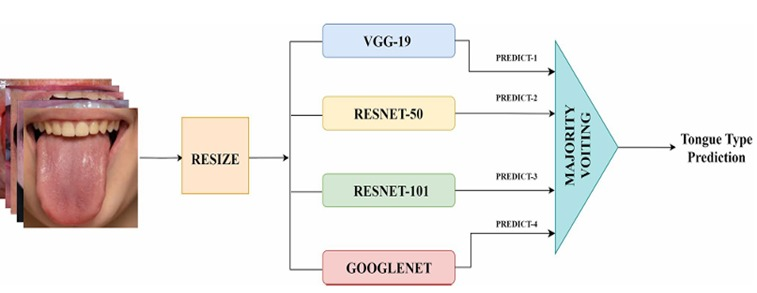
\includegraphics[width=0.85\textwidth]{2/figures/8.jpeg}
		\caption[Clasificación de lesiones linguales con DCNN y FBMV]{Estrategia de fusión por votación mayoritaria aplicada a modelos DCNN para clasificaciones binaria y multiclase. \\
		Fuente: \cite{Tiryaki2024}. \textit{Artificial intelligence in tongue diagnosis: classification of tongue lesions and normal tongue images using deep convolutional neural network.}}
		\label{2:fig130}
	\end{center}
\end{figure}

En conclusión, este trabajo destaca cómo la integración de DCNN y enfoques innovadores como FBMV puede transformar el diagnóstico de enfermedades bucales, proporcionando una base sólida para investigaciones futuras y desarrollos tecnológicos en medicina basada en imágenes.
